\documentclass[aspectratio=169]{beamer}
\setbeamertemplate{navigation symbols}{}
\usepackage{color,amsmath,comment, subfigure}
\usepackage{booktabs}
\usepackage{url}

%%%%%%%%%%%%%%%%%%%%%%%%%%
\title[]{Introduction}
\author[]{Matthew J. Salganik}
\institute[]{Social Networks (Soc 204)\\Princeton University}
\date[]{Wednesday, September 1, 2021\\ Week 1, Lecture 1

\vfill

\begin{flushleft}
\vspace{0.7in}

\includegraphics[width=0.05\textwidth]{figures/cc.png}
\end{flushleft}
}

\begin{document}
%%%%%%%%%%%%%%%%%%%%%%%%%%%
\frame{\titlepage}
%%%%%%%%%%%%%%%%%%%%%%%%%%%
\begin{frame}

\begin{center}
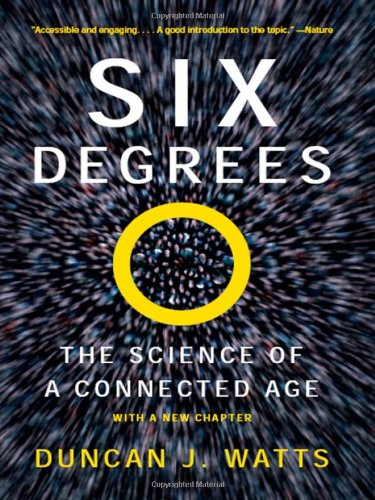
\includegraphics[height=0.50\textheight]{figures/watts_six_2003_cover}
\end{center}

\vfill

\begin{center}
\Large{
We live in the connected age.
}
\end{center}

\end{frame}
%%%%%%%%%%%%%%%%%%%%%%%%%%%
\begin{frame}

\begin{center}
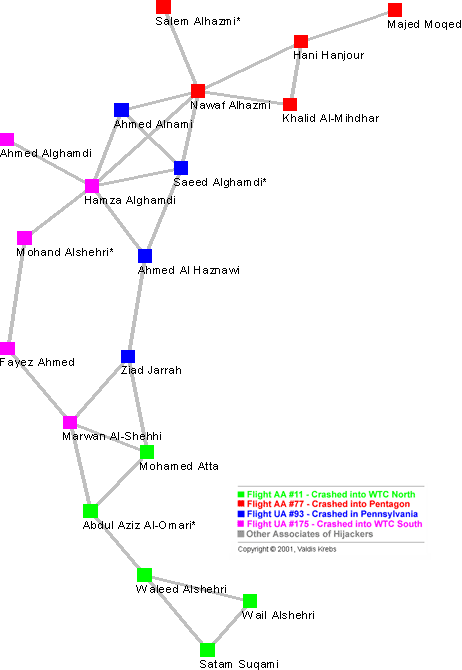
\includegraphics[height=0.90\textheight]{figures/krebs_uncloaking_2002_fig2}
\end{center}

\vfill
\Tiny{\url{http://pear.accc.uic.edu/ojs/index.php/fm/article/view/941/863}}

\end{frame}
%%%%%%%%%%%%%%%%%%%%%%%%%%%
\begin{frame}

\begin{center}
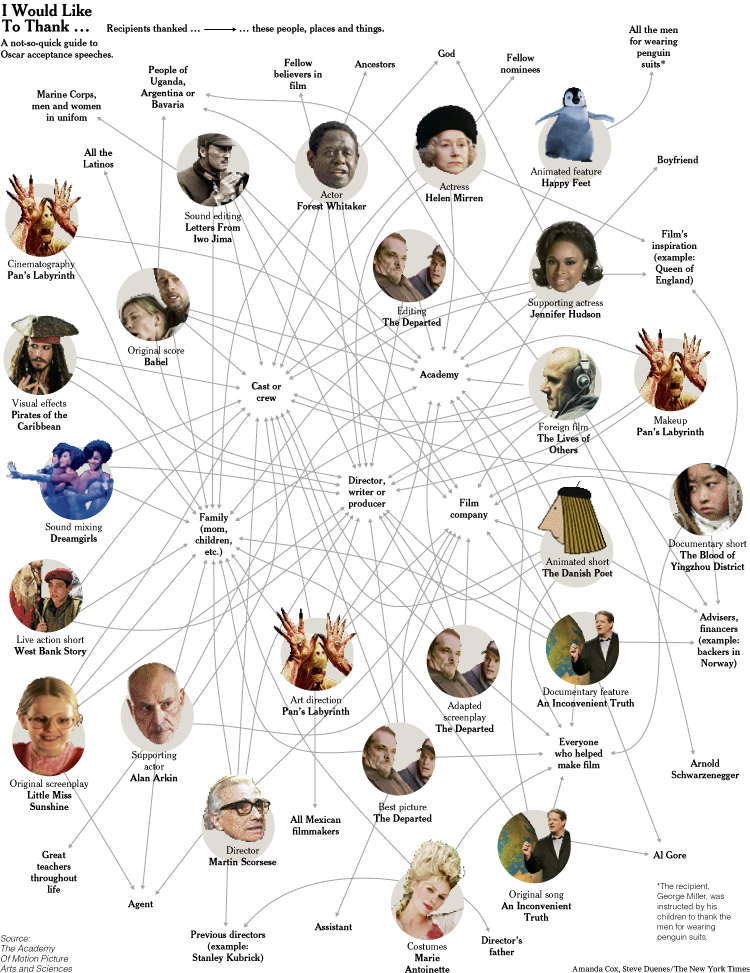
\includegraphics[height=0.9\textheight]{figures/nytimes_oscar_2007}
\end{center}

\vfill
\Tiny{\url{http://www.nytimes.com/imagepages/2007/02/26/movies/27graphic.ready.html}}

\end{frame}
%%%%%%%%%%%%%%%%%%%%%%%%%%%
\begin{frame}

\begin{center}
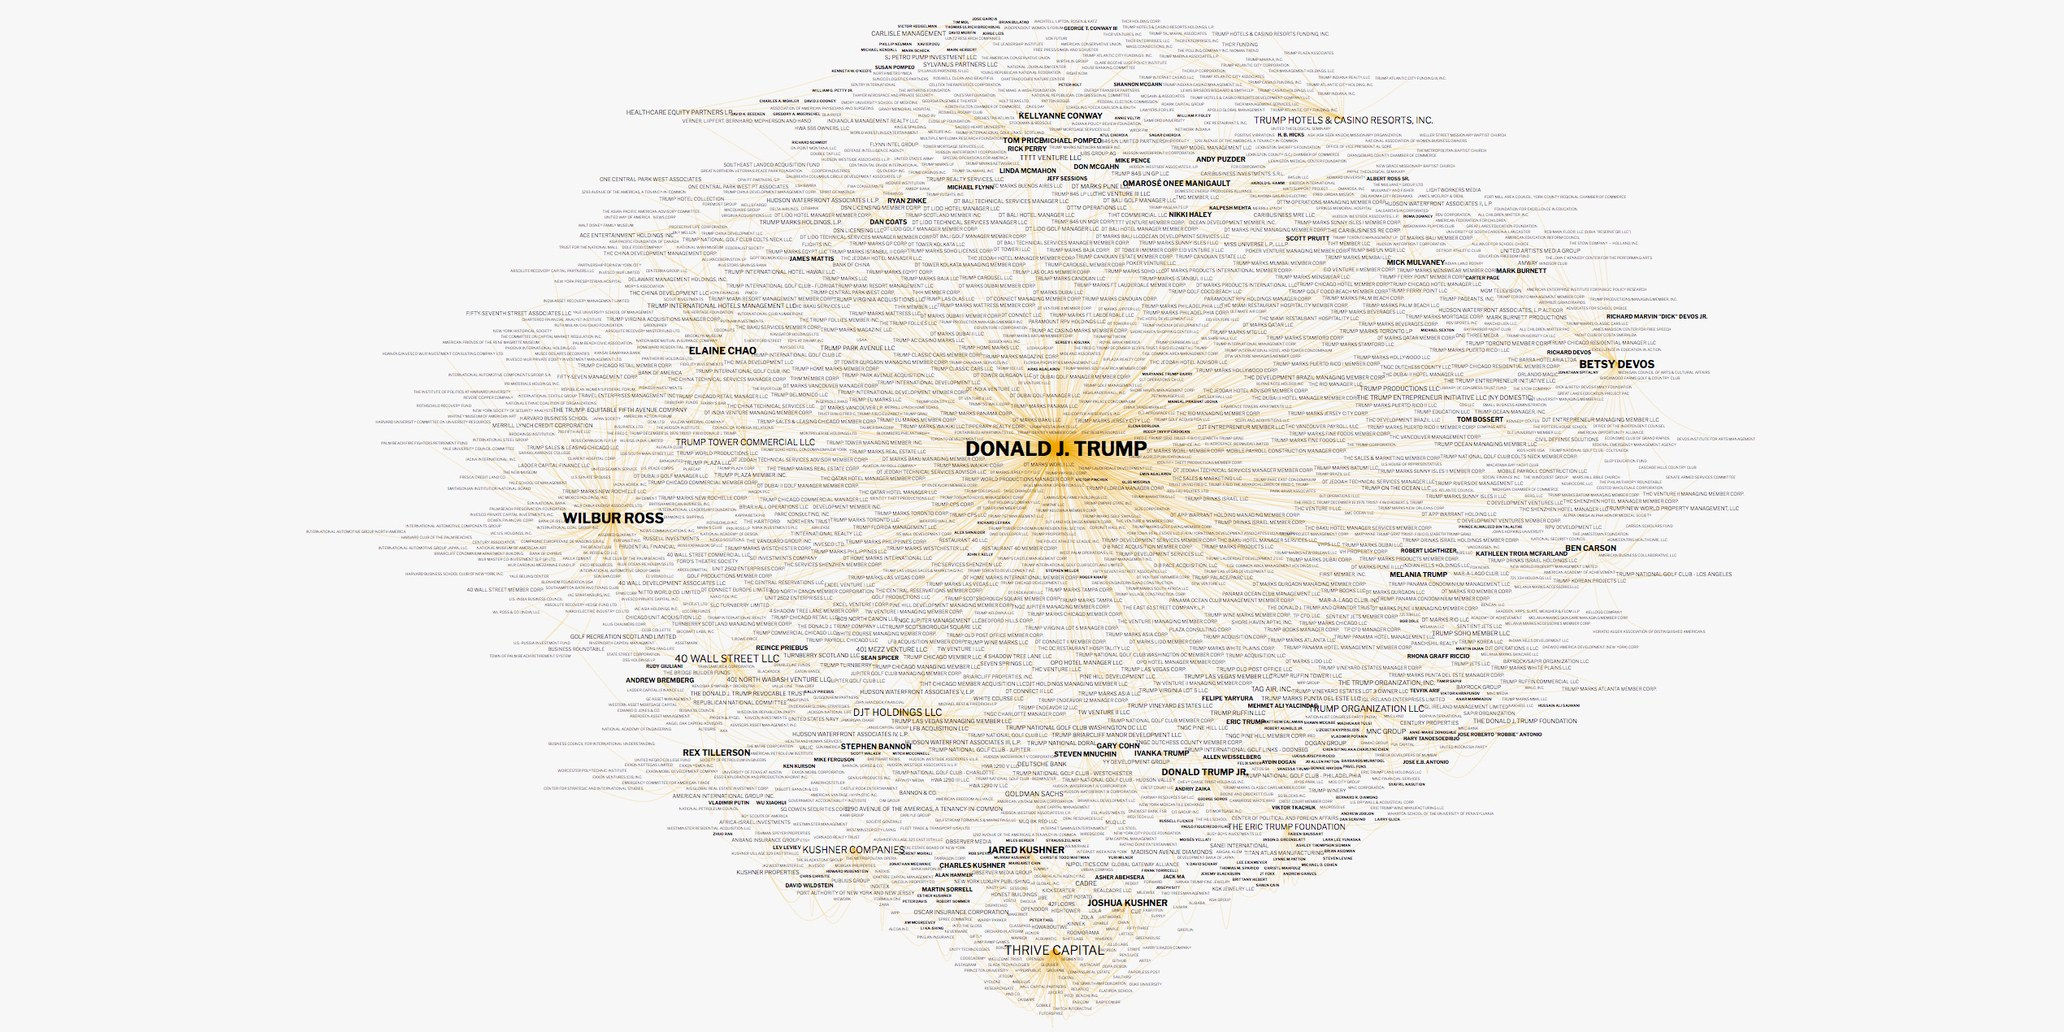
\includegraphics[width=0.9\textwidth]{figures/trump_network}
\end{center}

\vfill
\Tiny{\url{https://kimalbrecht.com/vis/\#trump-connections}}

\end{frame}
%%%%%%%%%%%%%%%%%%%%%%%%%%%
\begin{frame}

General pattern:
\begin{itemize}
\item nodes
\item edges
\end{itemize}

\end{frame}
%%%%%%%%%%%%%%%%%%%%%%%%%%%
\begin{frame}

\begin{center}
\Large{Your turn}
\end{center}

Think-pair-share: What are some other examples of networks? They don't need to be social.

\end{frame}
%%%%%%%%%%%%%%%%%%%%%%%%%%%
\begin{frame}

\begin{center}
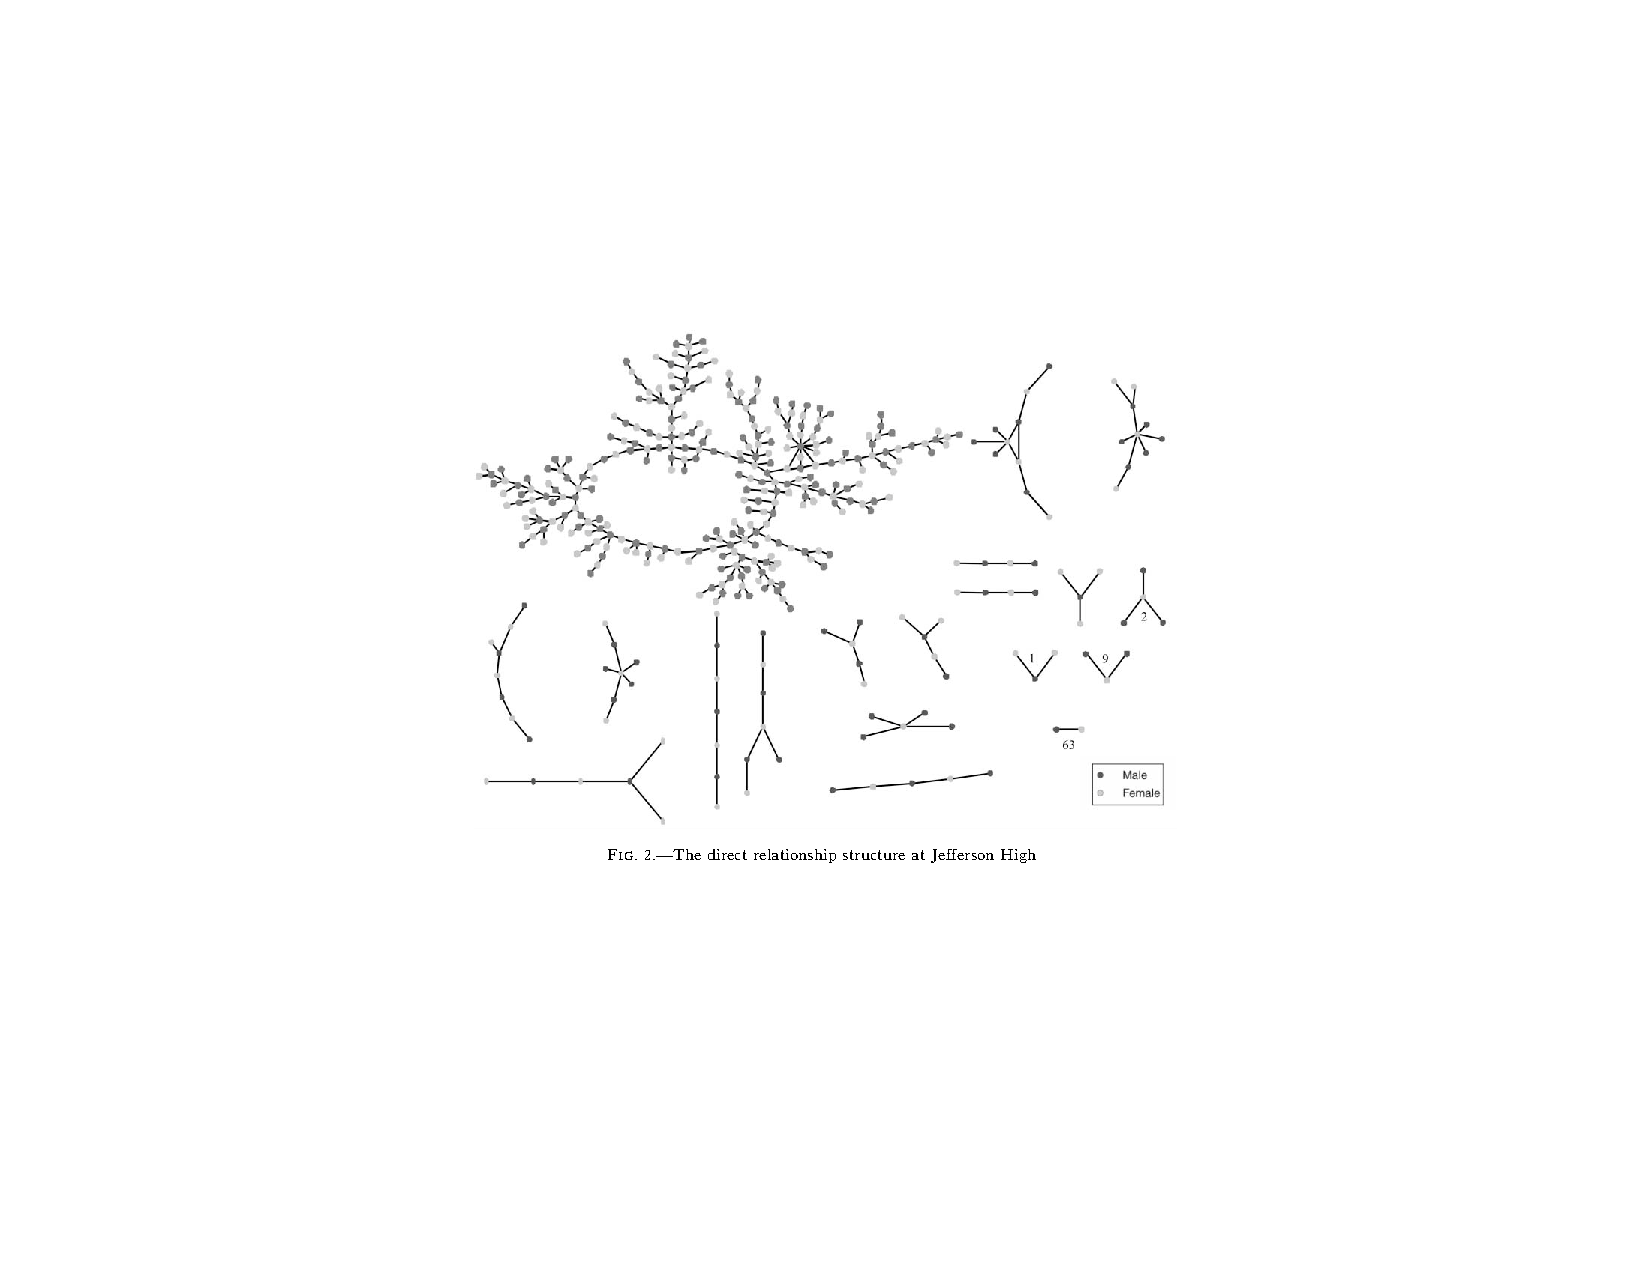
\includegraphics[width=0.95\textheight]{figures/bearman_chains_2004_fig2}
\end{center}

\vfill
\Tiny{url{http://www.journals.uchicago.edu/doi/10.1086/386272}}

\end{frame}
%%%%%%%%%%%%%%%%%%%%%%%%%%%
\begin{frame}
\frametitle{}

\setcounter{subfigure}{0}
\begin{figure}
  \centering
     \subfigure[American High School]{
     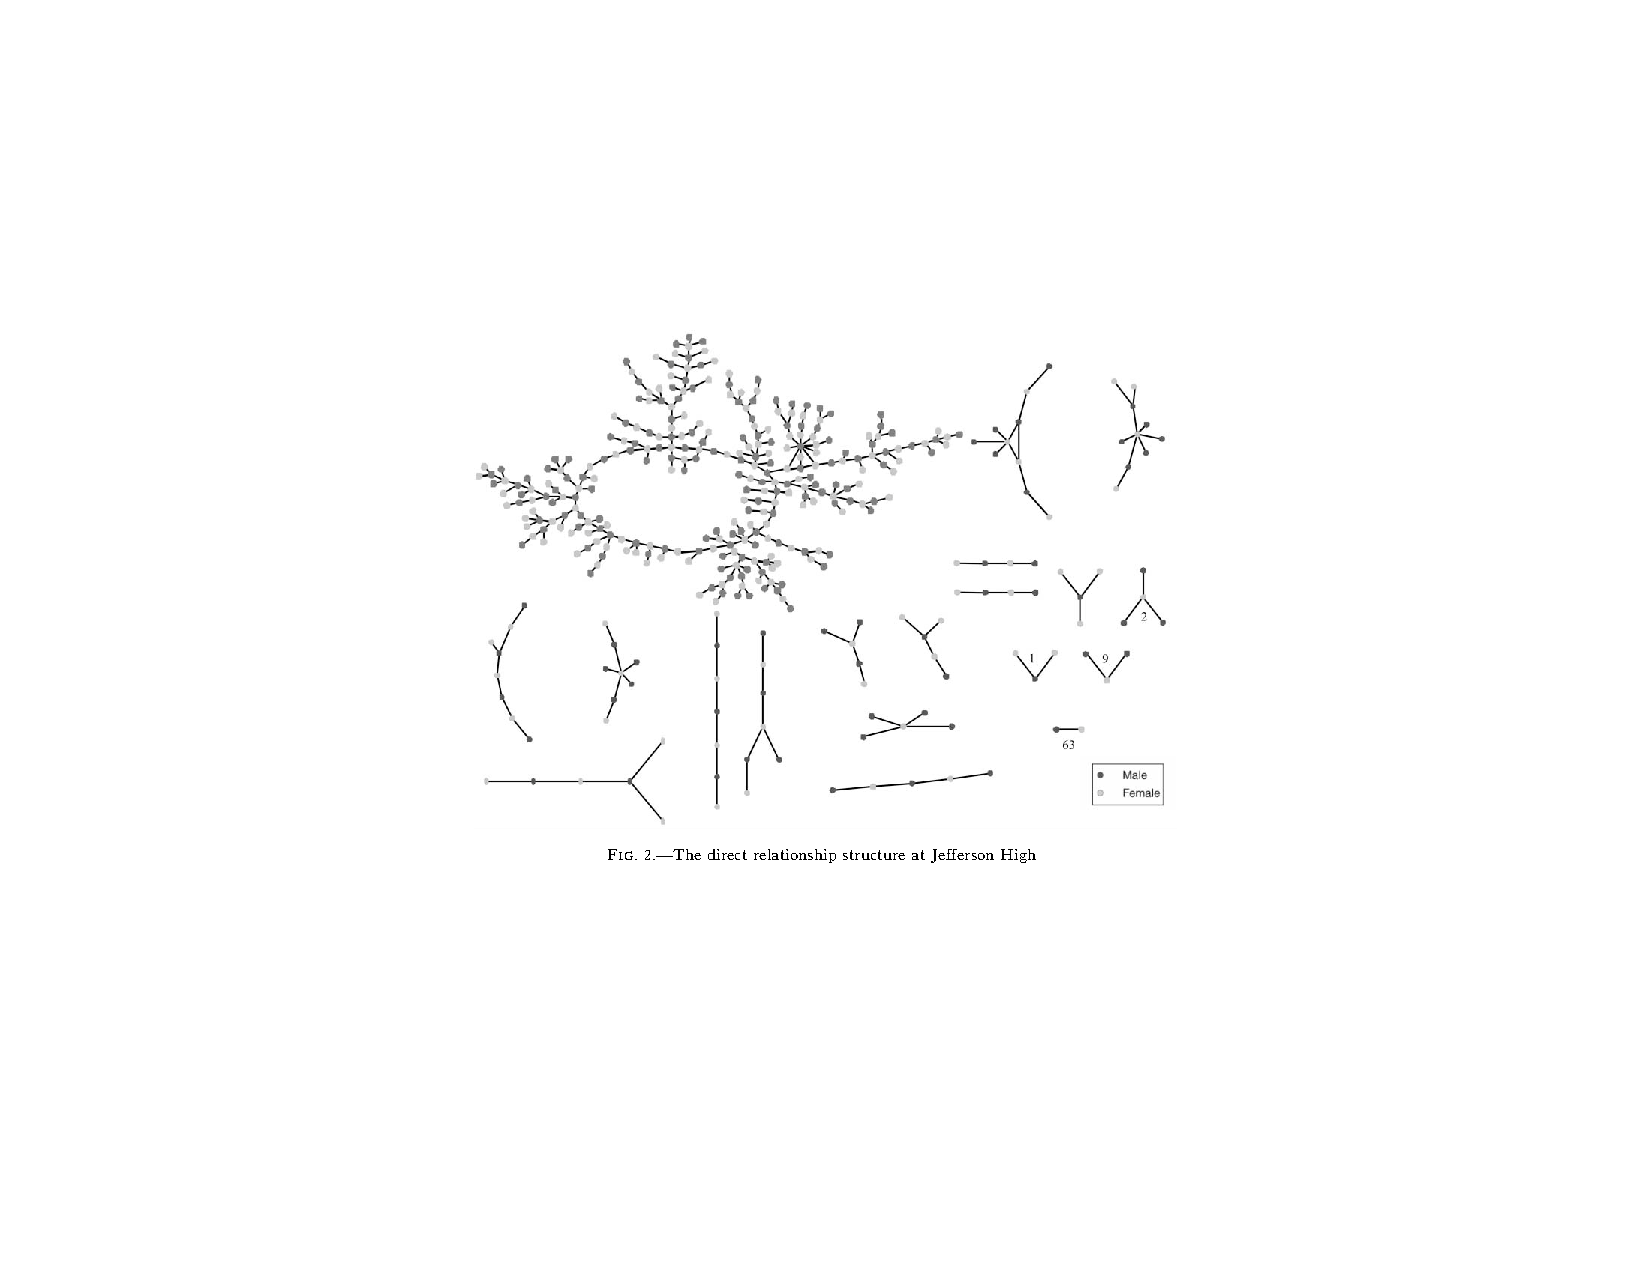
\includegraphics[width=0.45\textwidth]{figures/bearman_chains_2004_fig2}}
  \hspace{0in}
    \subfigure[Likoma Island, Malawi]{
    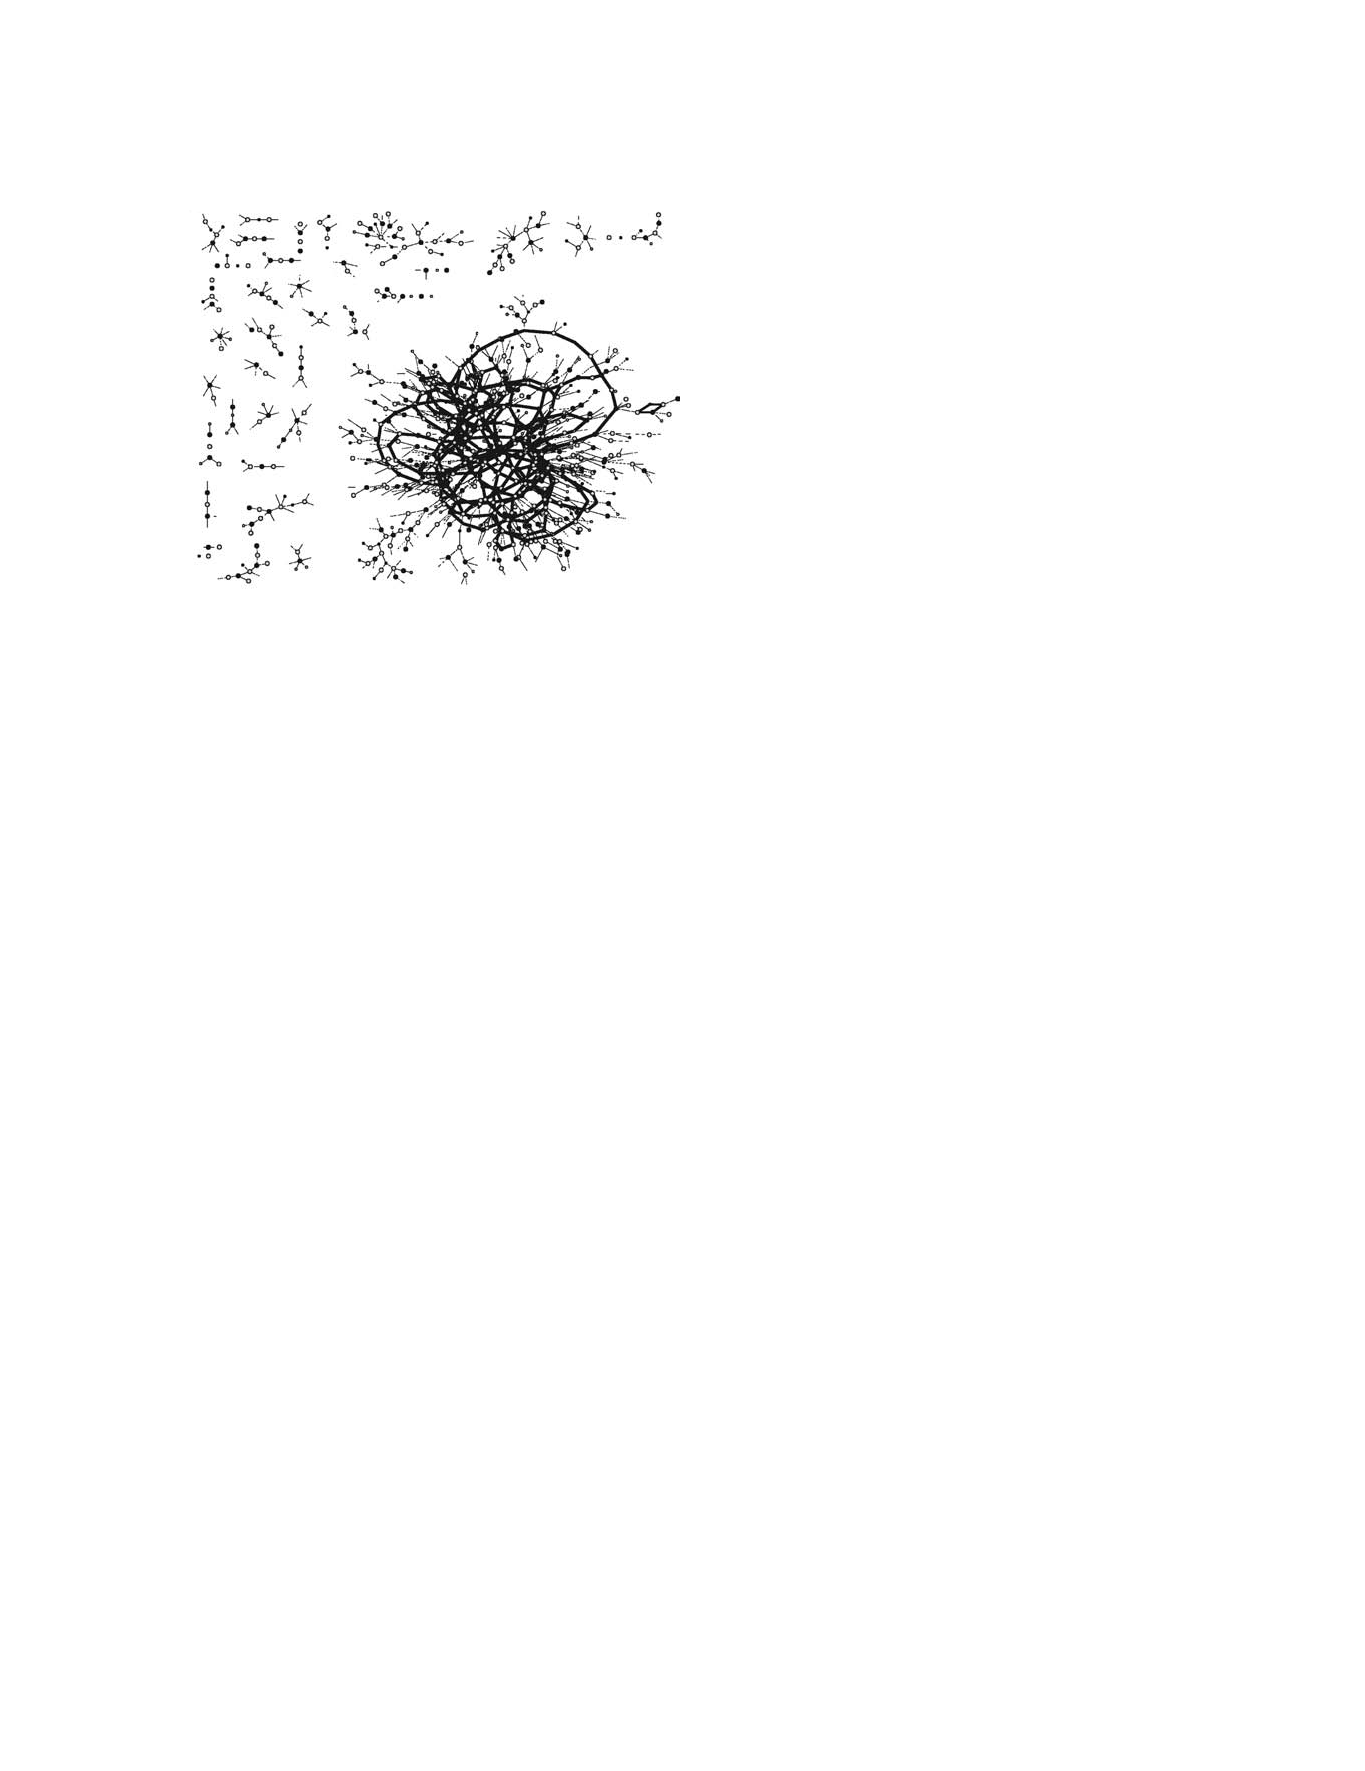
\includegraphics[width=0.45\textwidth]{figures/helleringer_sexual_2007_fig2a}}
\end{figure}

\vfill
\Tiny{\url{http://www.journals.uchicago.edu/doi/10.1086/386272} \& \url{https://www.ncbi.nlm.nih.gov/pubmed/18090281}}

\end{frame}
%%%%%%%%%%%%%%%%%%%%%%%%%%%
\begin{frame}

\begin{center}
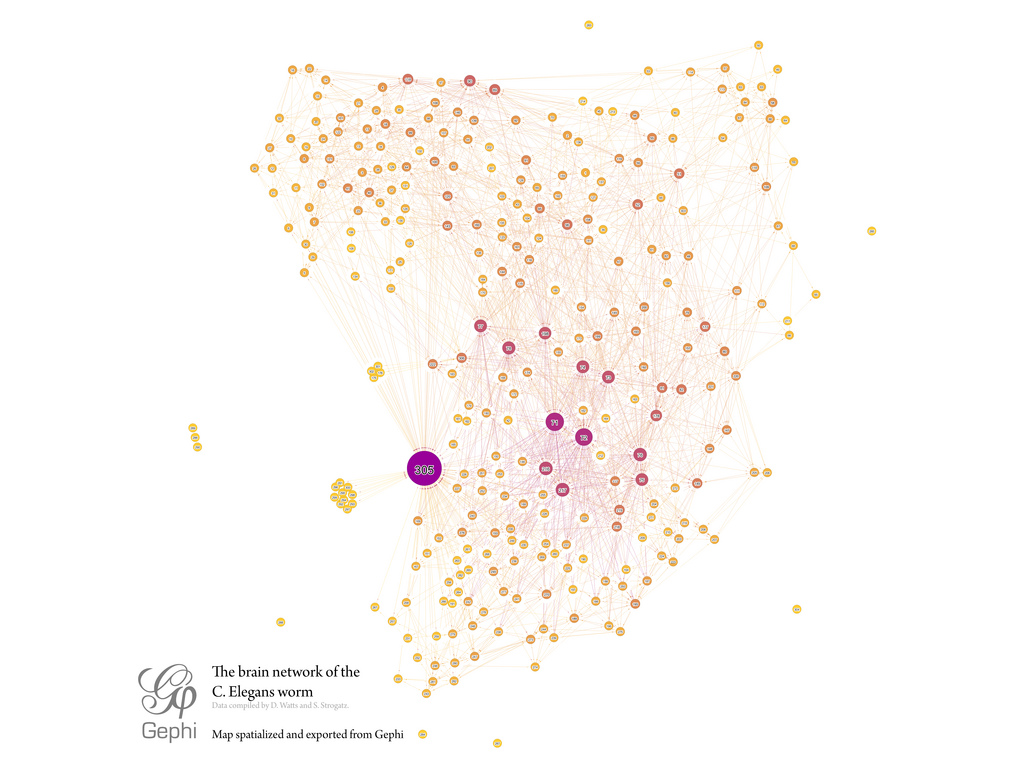
\includegraphics[height=0.9\textheight]{figures/celegans_brain_network}
\end{center}

\vfill
\Tiny{\url{https://commons.wikimedia.org/wiki/File:C.elegans-brain-network.jpg}}

\end{frame}
%%%%%%%%%%%%%%%%%%%%%%%
\begin{frame}
\frametitle{}

\setcounter{subfigure}{0}
\begin{figure}
  \centering
     \subfigure[Worm Brain]{
     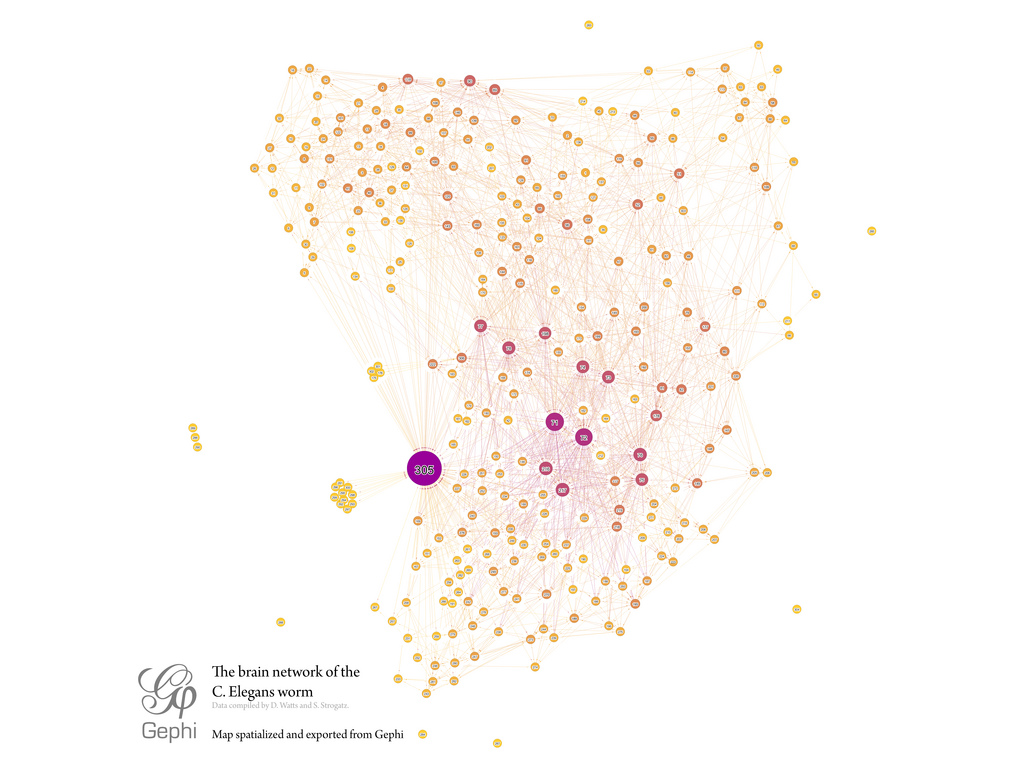
\includegraphics[width=0.45\textwidth]{figures/celegans_brain_network}}
  \hspace{0in}
    \subfigure[Power Grid]{
    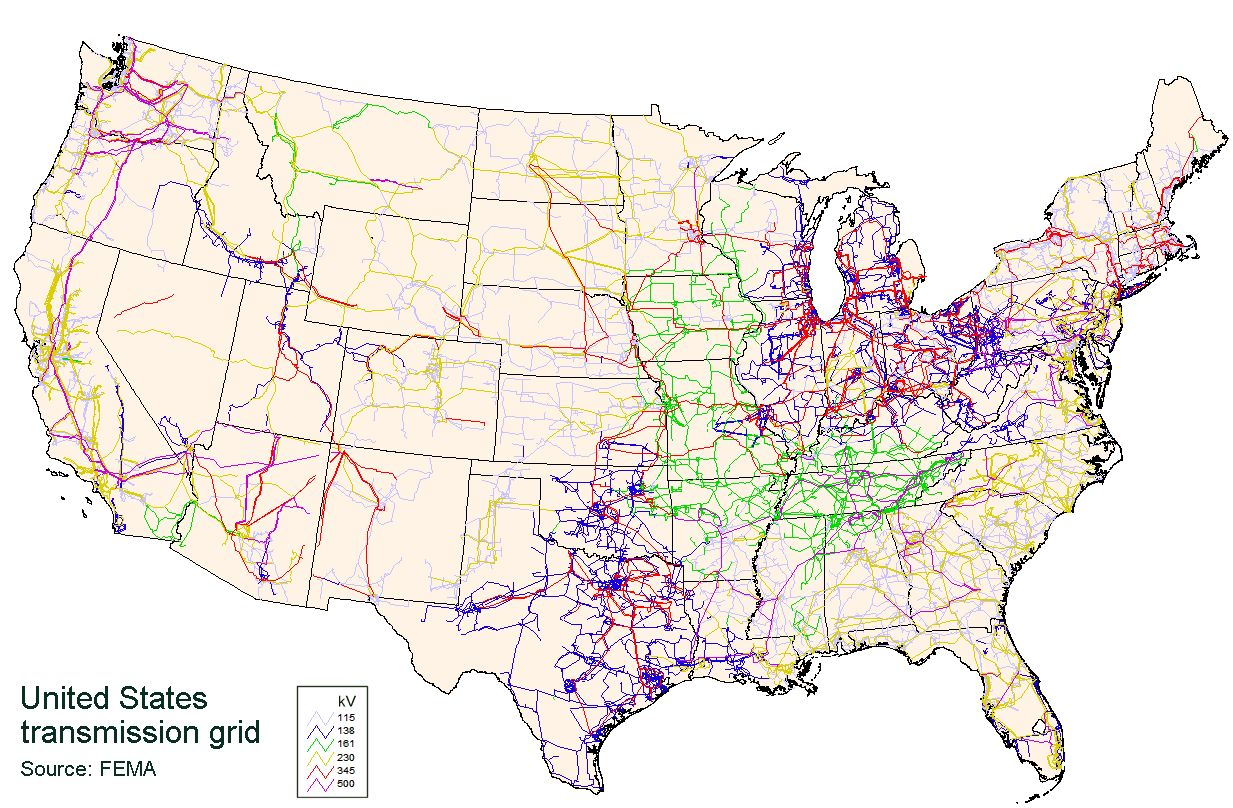
\includegraphics[width=0.45\textwidth]{figures/power_grid}}
\end{figure}

\vfill
\Tiny{\url{https://commons.wikimedia.org/wiki/File:C.elegans-brain-network.jpg} \& \url{https://commons.wikimedia.org/wiki/File:UnitedStatesPowerGrid.jpg}}

\note{
These two have similar structure
We will look not just a social networks but all kinds of networks
}

\end{frame}
%%%%%%%%%%%%%%%%%%%%%%%%%%%
\begin{frame}

\begin{center}
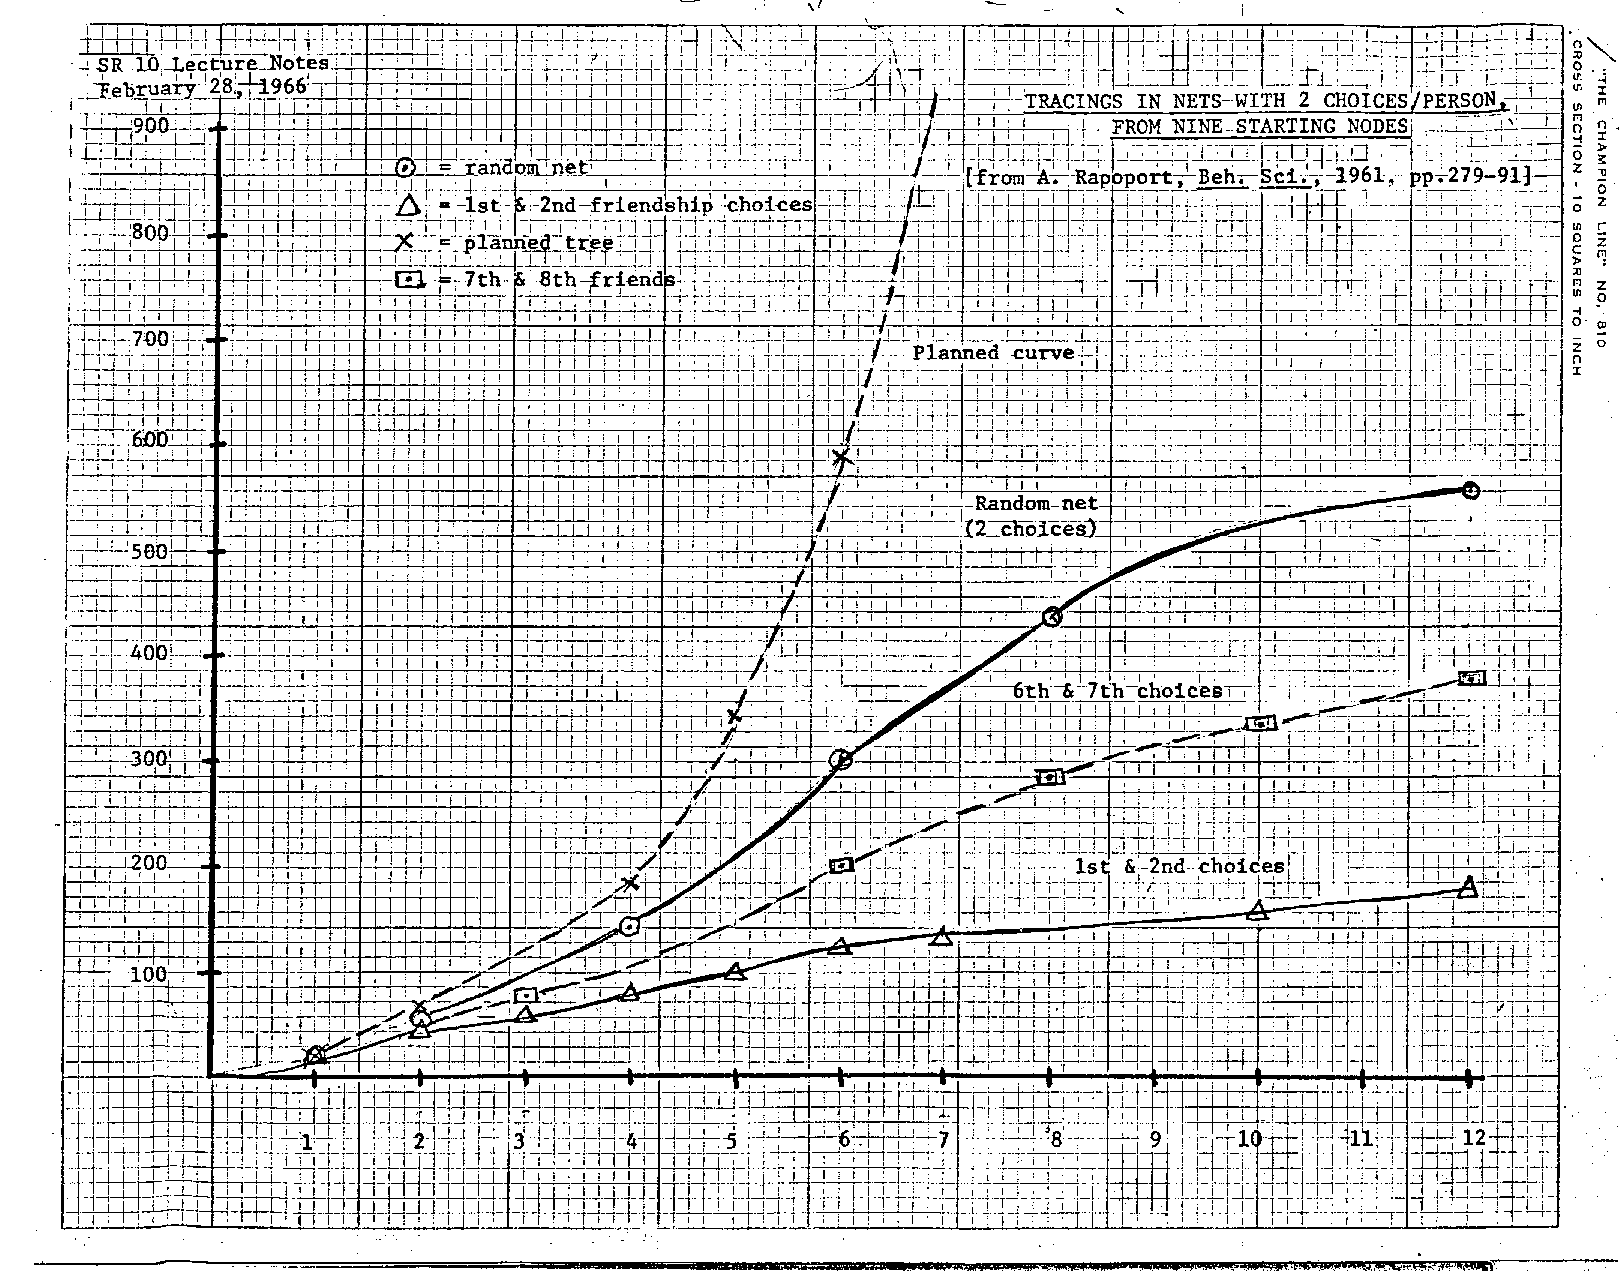
\includegraphics[height=0.9\textheight]{figures/white_classnotes_swt}
\end{center}

\note{
This is not a network in the same way as the others, but it summarizes data from a study from the 50s in middle school in Michigan
This is a graph is from a class taught at Harvard in 1966
This graph explains why you are more likely to get jobs from an acquaintances than close friends
Strength of weak ties
}

\end{frame}
%%%%%%%%%%%%%%%%%%%%%%%%%%%
\begin{frame}

\begin{center}
\Large{Learning objectives}
\end{center}

\end{frame}
%%%%%%%%%%%%%%%%%%%%%%%%%%%
\begin{frame}

\begin{itemize}
\item Students will be able to \textbf{describe} the major concepts used in the study of networks.
\pause
\item Students will be able to \textbf{describe} the interconnections between the major concepts used in the study of networks.
\pause
\item Students will be able to \textbf{use} the major concepts in the study of networks to gain insight into real-world phenomena.
\pause
\item Students will be able to \textbf{evaluate} real, modern research that connects the concepts of networks to real-world phenomena.
\end{itemize}

\end{frame}
%%%%%%%%%%%%%%%%%%%%%%%%%%%
\begin{frame}

\begin{center}
\Large{Major activities}
\end{center}

\end{frame}
%%%%%%%%%%%%%%%%%%%%%%%%%%%
\begin{frame}

\begin{center}
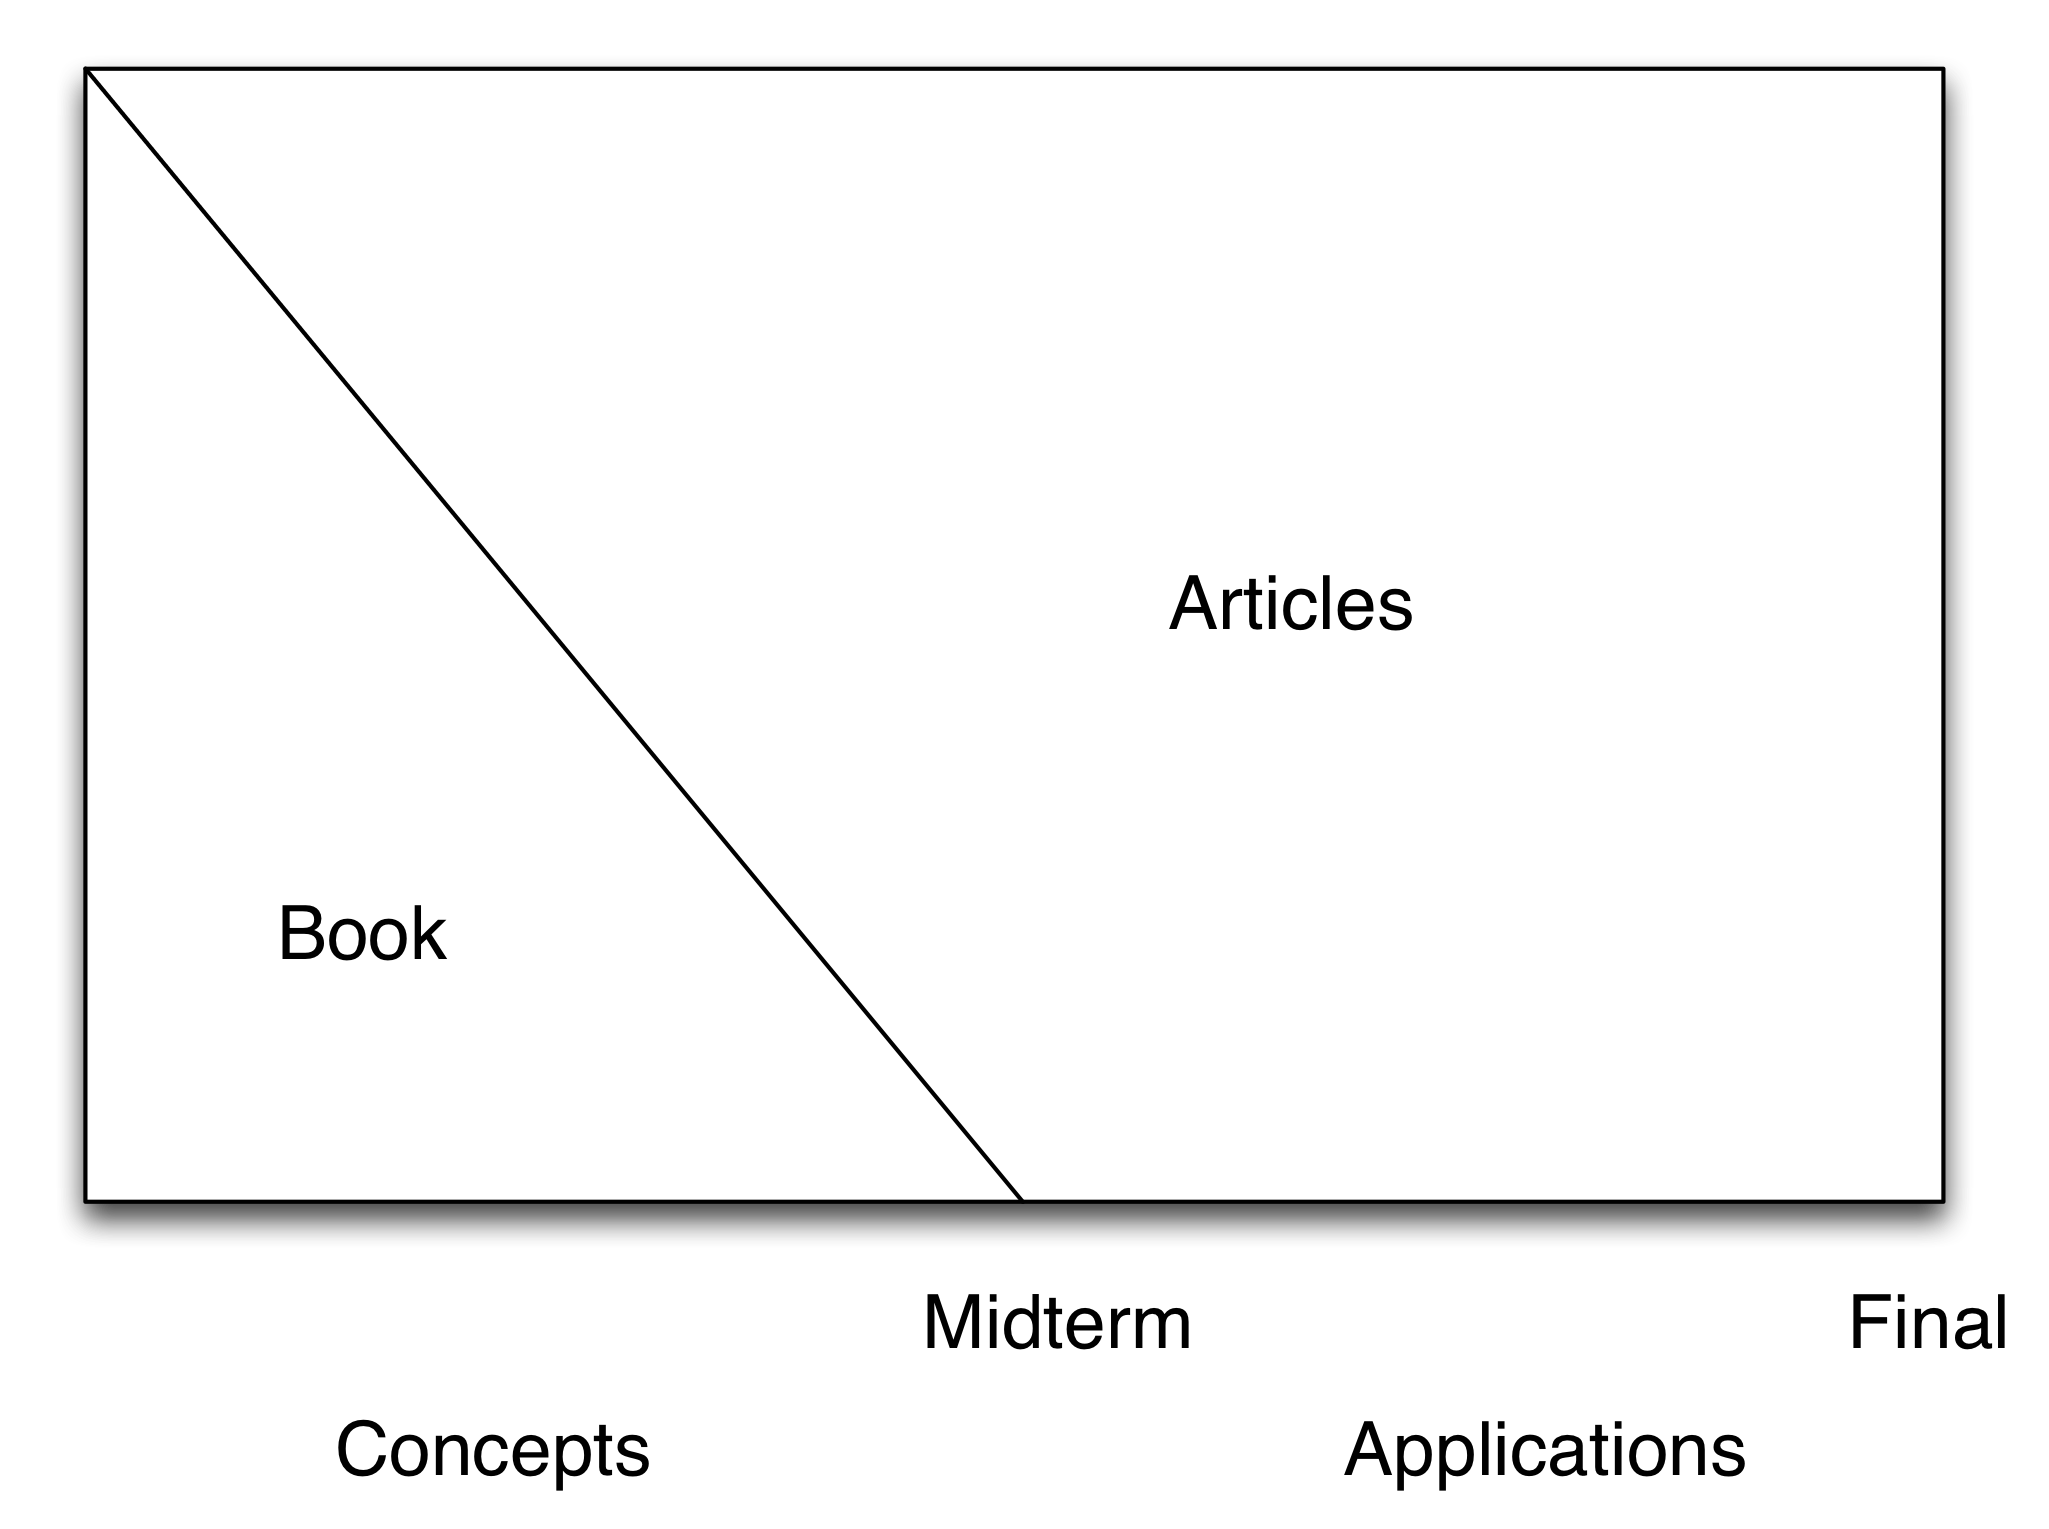
\includegraphics[height=0.90\textheight]{figures/class_structure}
\end{center}

\note{
Not a thriller move that leads up to one big climax, more like a corkscrew that winds around
}

\end{frame}
%%%%%%%%%%%%%%%%%%%%%%%%%%%
\begin{frame}

\begin{itemize}
\item Weekly precept assignment
\item Weekly quiz
\item Midterm exam
\item Final exam
\end{itemize}

\end{frame}
%%%%%%%%%%%%%%%%%%%%%%%%%%%
\begin{frame}

Each week
\begin{itemize}
\item Watch pre-read video
\pause
\item Do reading
\pause
\item Come to lecture
\pause
\item Watch pre-read video
\item Do reading
\item Submit quiz on Canvas
\item Submit weekly assignment
\item Come to lecture
\pause
\item Attend precept
\end{itemize}

\end{frame}
%%%%%%%%%%%%%%%%%%%%%%%%%%%%
\begin{frame}
\frametitle{Example assignment}

\begin{center}
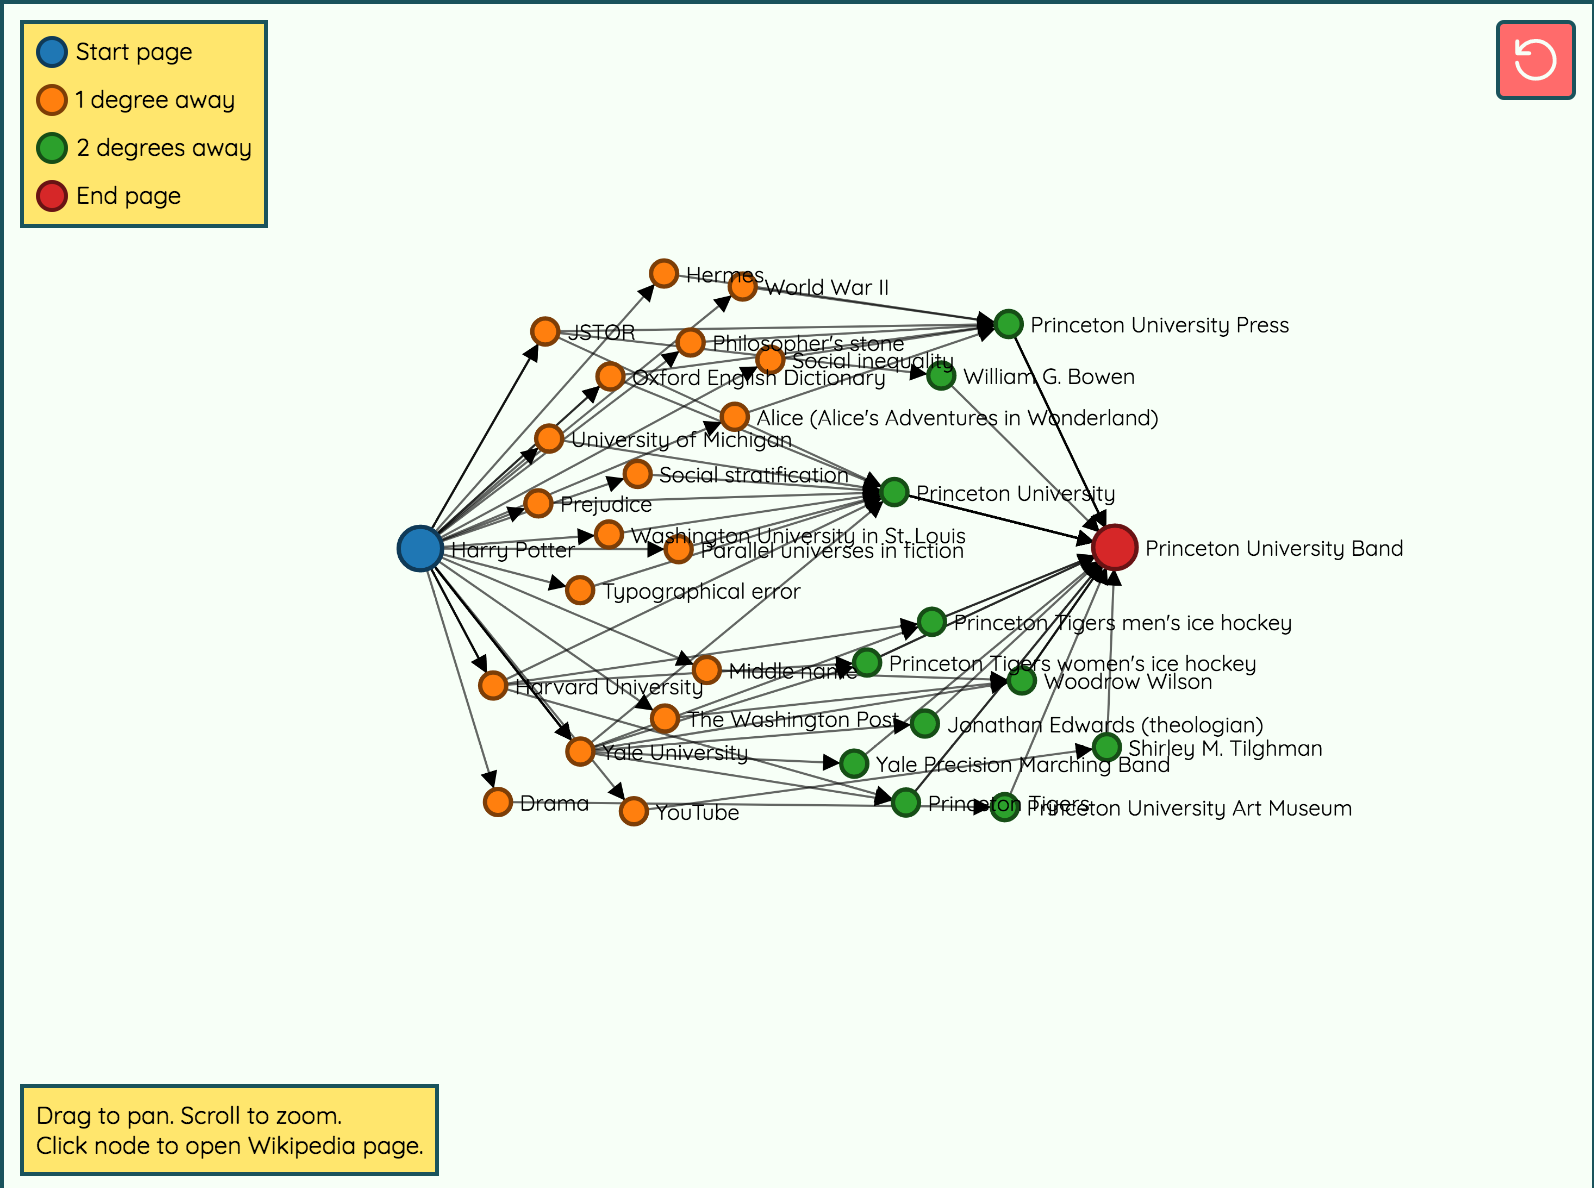
\includegraphics[height=0.9\textheight]{figures/six_degrees_wikipedia_example}
\end{center}

\vfill
\Tiny{\url{https://www.sixdegreesofwikipedia.com/?source=Harry\%20Potter&target=Princeton\%20University\%20Band}}

\end{frame}
%%%%%%%%%%%%%%%%%%%%%%%%%%%
\begin{frame}
\frametitle{Example assignment}

\begin{center}

\includegraphics[width=0.95\textwidth]{figures/kramer_experimental_2014_title}
\end{center}

\vfill
\Tiny{\url{https://doi.org/10.1073/pnas.1320040111}}

\end{frame}
%%%%%%%%%%%%%%%%%%%%%%%%%%%
\begin{frame}
\frametitle{Example assignment}

\begin{center}
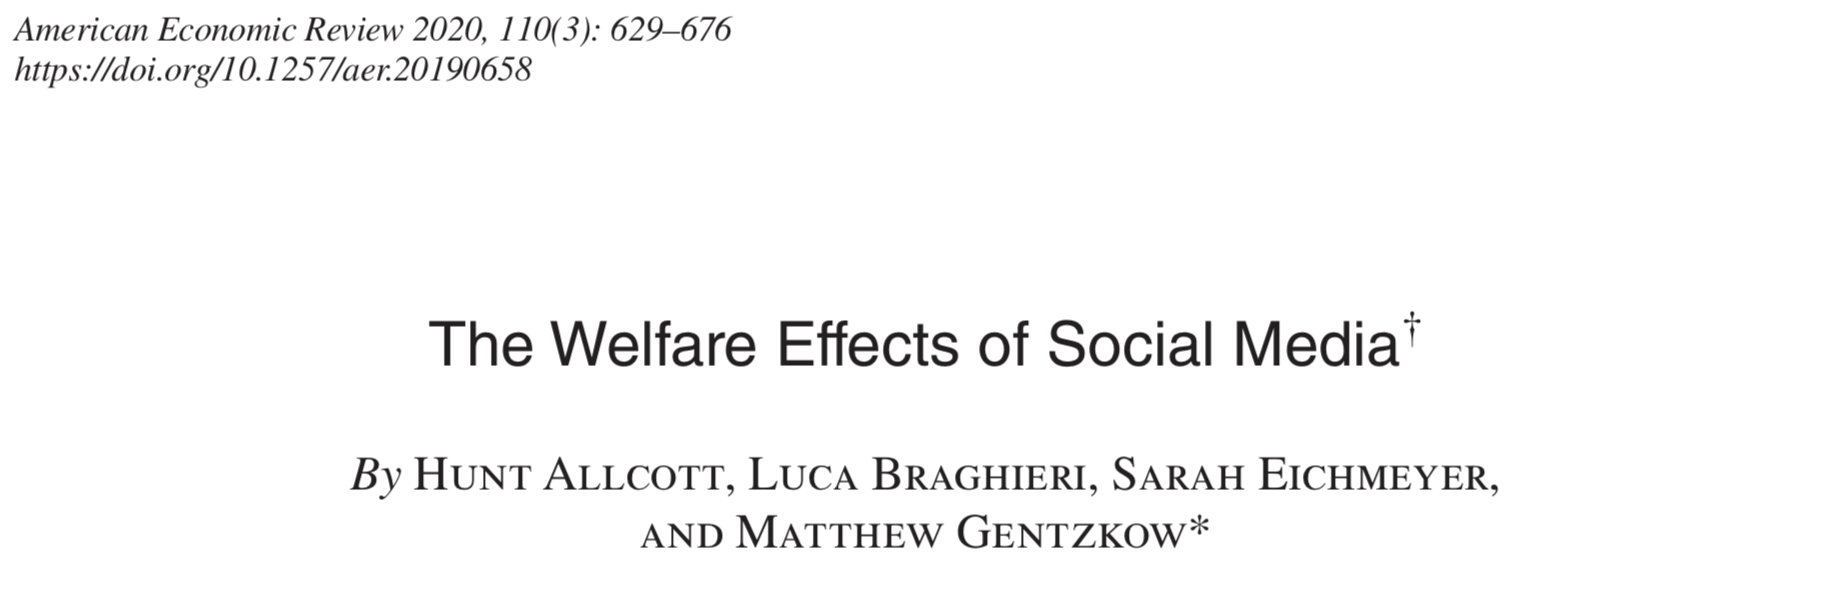
\includegraphics[width=0.95\textwidth]{figures/allcott_welfare_2020_title}
\end{center}

\vfill
\Tiny{\url{https://doi.org/10.1257/aer.20190658}}

\end{frame}
%%%%%%%%%%%%%%%%%%%%%%%%%%%
\begin{frame}
\frametitle{Precept philosophy}

\begin{center}

\includegraphics[height=0.80\textheight]{figures/princeton_precept}
\end{center}

\vfill
\Tiny{\url{http://www.princeton.edu/pr/pub/precept/PU-Inspired-Conversations-2008.pdf}}

\note{
Precepts started in 1905
Precept is a time for active learning
You can of course use this time to ask questions, but you should expect to learn new things not just hear a rehash of the lecture
}

\end{frame}
%%%%%%%%%%%%%%%%%%%%%%%%%%%
\begin{frame}

\begin{center}
\Large{Getting to know each other}
\end{center}

\end{frame}
%%%%%%%%%%%%%%%%%%%%%%%%%%%
\begin{frame}

\begin{center}
\Large{About me}
\end{center}

\end{frame}
%%%%%%%%%%%%%%%%%%%%%%%%%%%
\begin{frame}

About the preceptors:
\begin{itemize}
\item Emily Cantrell
\item Katie Donnelly-Moran
\item Max Fineman
\end{itemize}

\end{frame}
%%%%%%%%%%%%%%%%%%%%%%%%%%%
\begin{frame}

\begin{center}
\Large{About you}
\end{center}

\end{frame}
%%%%%%%%%%%%%%%%%%%%%%%%%%%
\begin{frame}

\begin{itemize}
\item first year, second year, third year, fourth year
\pause
\item no major, sociology, social science (but not sociology), humanities, natural sciences, cs/engineering
\end{itemize}

\end{frame}
%%%%%%%%%%%%%%%%%%%%%%%%%%%
\begin{frame}

\begin{center}
\includegraphics<1>[width=0.5\textwidth]{figures/fb_logo} %
\includegraphics<2>[width=0.5\textwidth]{figures/instagram_logo} %
\includegraphics<3>[width=0.5\textwidth]{figures/twitter_logo} %
\includegraphics<4>[width=0.5\textwidth]{figures/tiktok_logo} %
\includegraphics<5>[width=0.40\textwidth]{figures/yikyak_logo} %
\includegraphics<6>[width=0.35\textwidth]{figures/questionmark} %
\end{center}

have account, active user (6 of past 7 days)

\end{frame}
%%%%%%%%%%%%%%%%%%%%%%%%%%%
\begin{frame}
\frametitle{More information about the course}

Logistical notes:
\begin{itemize}
\item We will post an announcement on Canvas when precept times are set
\item There is no precept this week
\item There is no quiz this week
\end{itemize}

\end{frame}
%%%%%%%%%%%%%%%%%%%%%%%%%%%
\begin{frame}
\frametitle{More information about the course}

\begin{itemize}
\item Canvas, especially modules page: {\tiny \url{https://princeton.instructure.com/courses/4801/modules}}
\pause
\item Additional information about readings: {\tiny \url{https://www.princeton.edu/~mjs3/soc204_f2021/readings.shtml}}
\pause
\item Additional information about class logistics: {\tiny \url{https://www.princeton.edu/~mjs3/soc204_f2021/logistics.shtml}}
\end{itemize}

\note{
I expect you to read syllabus
}

\end{frame}
%%%%%%%%%%%%%%%%%%%%%%%%%%%%
\begin{frame}

\begin{center}
\Large{Is this course right for you?}
\end{center}

\note{
Working hard, weekly assignments, difficult reading
Support you need to be successful
For students in social science and humanities more mathematical, different reading
For computer science engineering students, more reading, different reading
}

\end{frame}
%%%%%%%%%%%%%%%%%%%%%%%%%%%
\begin{frame}

\begin{center}
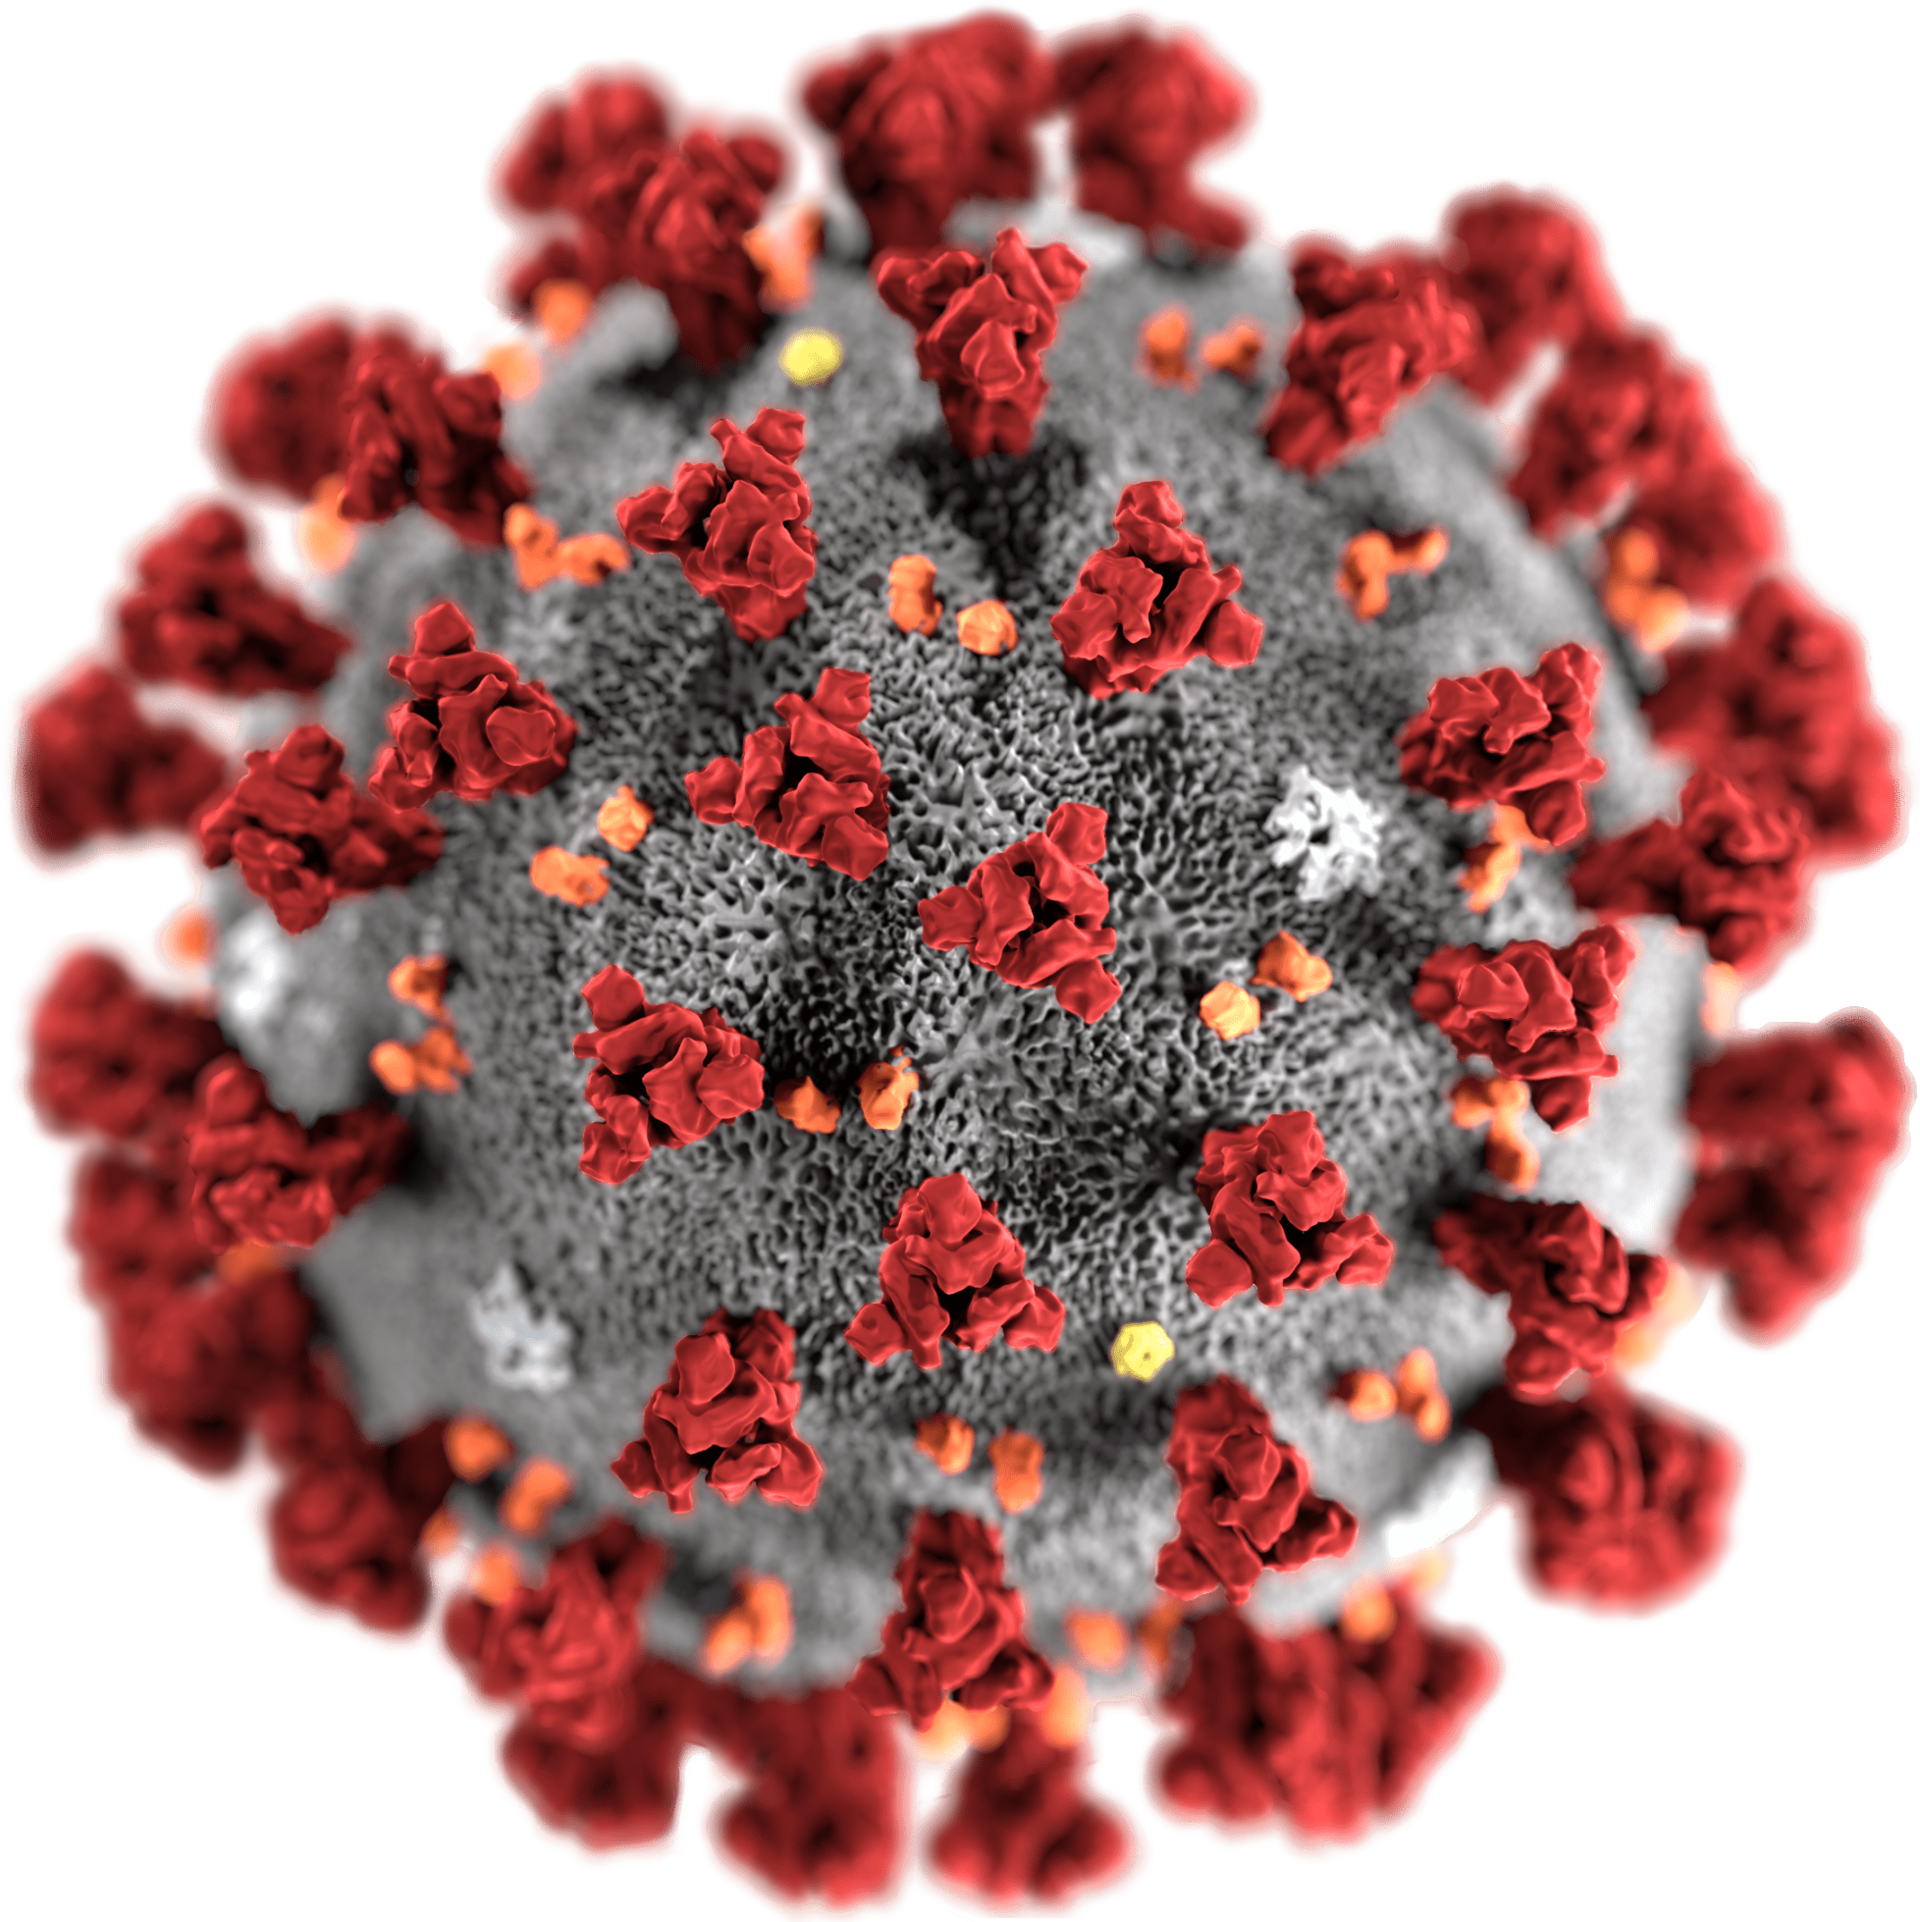
\includegraphics[height = 0.9\textheight]{figures/covid}
\end{center}

\vfill
\tiny{\url{https://phil.cdc.gov/Details.aspx?pid=23312}}

\note{
COVID, hard time for me and my family, hard time for everyone
If you are having trouble physically or mentally support is available.
We will follow university guidelines
This course is about how we are connected, and COVID shows how our health is connected
}

\end{frame}
%%%%%%%%%%%%%%%%%%%%%%%%%%%%
\begin{frame}

Next class: The connected age and the small world problem

\end{frame}
%%%%%%%%%%%%%%%%%%%%%%%%%%%




\end{document}
